\chapter{Gerenciamento do projeto}
\label{chap:metodologia}

    Ao iniciar o desenvolvimento de um novo projeto, é primordial definir um plano com etapas estabelecidas a fim de alcançar os objetivos gerais. Nesse sentido, a organização de prazos, o levantamento de compreensão dos papéis ocupados por cada integrante dentro da equipe, a designação de tarefas e a gestão de entregas constituem aspectos fundamentais para garantir um projeto final robusto e completo. Portanto, definir ferramentas e metodologias para guiar o gerenciamento desses aspectos mostra-se relevante para manter um progresso contínuo e sem conflitos.


\section{Metodologias e Ferramentas de Gestão de Projeto}\label{sec:exemplo-de-algoritmos-e-figuras}

    Com o propósito de manter entregas constantes e estabelecer um acesso fácil a todos os aspectos do projeto, decidiu-se utilizar as ferramentas fornecidas pela Atlassian devido às funcionalidades ofertadas e, sobretudo, pela centralização das informações e integração entre as diferentes plataformas. As plataformas são gratuitas para equipes com até dez membros, promovendo um alto custo-benefício ao grupo. 

    \subsection{Jira}
    
    O Jira foi estabelecido como a principal maneira de organizar e designar tarefas entre os integrantes do grupo. Por promover a possibilidade de visualizar itens pendentes em linhas do tempo, segmentar entregas semanais em tarefas atômicas e fornecer uma visão unificada de tudo que está pendente, em progresso ou concluído, a plataforma facilita a gestão eficiente do fluxo de trabalho.
    
    Além disso, a ferramenta permite que a equipe crie campos personalizados para atender às necessidades do projeto, acesse diferentes dashboards e utilize filtros para visualizações de diferentes aspectos do projeto. Com relatórios e métricas detalhadas, o Jira também oferece dados sobre o progresso do projeto, ajudando a identificar áreas de melhoria e de sucesso, auxiliando a tomar decisões informadas para impulsionar o sucesso do projeto.

    Por fim, o Jira oferece recursos adicionais, como a atribuição de prazos, a adição de descrições detalhadas às tarefas e a possibilidade de anexar arquivos relevantes, como documentos ou imagens. Isso contribui para uma comunicação mais eficiente entre os membros da equipe e auxilia na documentação do processo de desenvolvimento.

    \subsection{Adaptação do framework Scrum}

    O framework Scrum, conhecido por sua agilidade e flexibilidade, foi adaptado para se adequar ao contexto específico do projeto, levando em consideração a disponibilidade dos integrantes do grupo. Ao invés de adotar sprints com períodos de tempo fixos, decidiu-se estabelecer o ritmo de trabalho com base nos dias em que ocorrem as entregas em sala de aula. Essa abordagem permite uma melhor sincronização das atividades com o calendário acadêmico, garantindo que todas as tarefas estejam concluídas a tempo para as avaliações.

    Embora as aulas aconteçam semanalmente, as entregas podem ser espaçadas por períodos maiores, a depender do calendário acadêmico. Assim, optamos por agrupar todas as atividades necessárias para alcançar o objetivo da próxima entrega, independentemente do intervalo de tempo entre elas. Essa estratégia permite uma alocação mais eficiente de tempo e recursos, pois é possível focar nas tarefas mais relevantes e críticas para o avanço do projeto. Além disso, ao definir as sprints baseadas em entregas, viabiliza-se conversas com o professor durante as aulas anteriores à apresentação com o propósito de tirar dúvidas, refinar detalhes e coletar feedbacks sobre o andamento do projeto.
    
    No Jira, utilizamos a divisão por épicos para organizar e priorizar as diversas etapas e funcionalidades do projeto. Essa categorização nos permite visualizar de forma clara e detalhada todas as atividades que precisam ser realizadas até a data limite estabelecida. Com isso, podemos planejar e executar as tarefas de forma estratégica, mantendo o foco no cumprimento dos objetivos e na entrega bem-sucedida do projeto. Ademais, cada tarefa, sub-tarefa e história pode ser designada aos integrantes.

    \begin{figure}[h!]
        \captionsetup{width=1\textwidth} 
        \caption{\label{fig:epicos_jira} Divisão por épicos para organização de entregas}
        \centering
        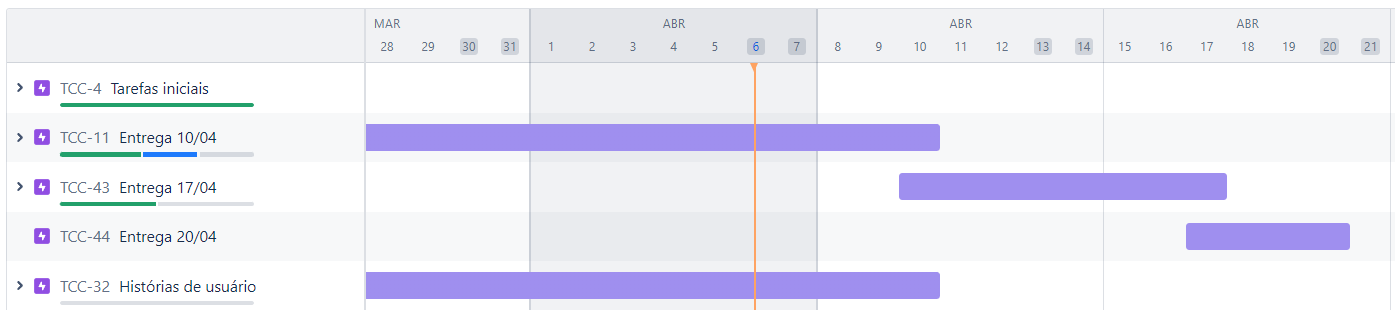
\includegraphics[width=1\textwidth]{figuras/epicos_jira}
        \caption*{Fonte: elaborada pelo autor.}
    \end{figure}

    A Figura \ref{fig:epicos_jira} ilustra a divisão por épicos, sendo que cada um constitui uma data de entrega. Assim, o intervalo de tempo das entregas ficam facilmente visíveis. 

    
    \subsection{Kanban}
    No contexto do projeto, a ferramenta de administração de produção Kanban foi adotada para facilitar o gerenciamento visual das tarefas, prioridades e fluxo de trabalho da equipe. O Kanban é uma metodologia ágil que se baseia em quadros visuais divididos em colunas que representam diferentes estágios do processo de trabalho. Cada tarefa é representada por um cartão, que é movido pelas colunas conforme progride no fluxo de trabalho.

    No presente projeto, a ferramenta Kanban foi implementada utilizando o Jira, uma plataforma que oferece recursos específicos para a criação e personalização de quadros Kanban. Esses quadros podem ser adaptados de acordo com as necessidades da equipe, permitindo a definição de colunas correspondentes aos estágios específicos do processo de desenvolvimento de software, como "A fazer", "Em andamento"  e "Concluído". A atualização das tarefas nos quadros é refletida instantaneamente quando o estado do trabalho é atualizado, evitando duplicação de itens em diferentes lugares, como ilustra a Figura \ref{fig:kanban}.
    
    A exibição dos itens nos quadros pode ser filtrada por épicos, mostrando a situação das tarefas de cada entrega, e também pode ser agrupada por épico, subtarefa ou responsável. Essas funcionalidades disponibilizadas pela plataforma facilitam o acompanhamento do progresso do projeto e permitem uma visão clara e organizada das atividades em andamento.

    \begin{figure}[h!]
        \captionsetup{width=1\textwidth}
        \caption{\label{fig:kanban} Quadros do Kanban disponibilizados no Jira}
        \centering
        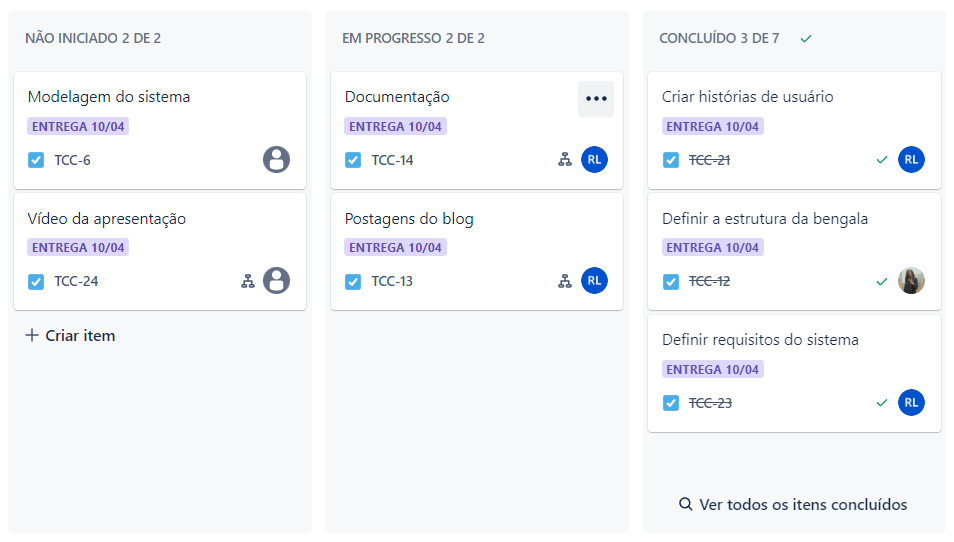
\includegraphics[width=1\textwidth]{figuras/kanban} 
        \caption*{Fonte: elaborada pelo autor.}
    \end{figure}

    \subsection{Github e Git}

    O GitHub, uma plataforma de hospedagem de arquivos baseada no sistema de versionamento Git, é uma ferramenta amplamente reconhecida e adotada pela comunidade de desenvolvimento de software. Sua popularidade se deve à sua capacidade de gerenciar alterações e facilitar a colaboração entre equipes de desenvolvimento. Para o projeto, a escolha do GitHub foi natural, uma vez que todos os membros já possuíam familiaridade com a plataforma.
    
    O Git, por sua vez, é um sistema de versionamento distribuído que permite que os membros de um projeto clonem o repositório, realizem alterações localmente e abram solicitações para mesclar essas mudanças na versão principal existente no repositório. Uma das principais vantagens do Git é sua capacidade de lidar com conflitos de maneira eficiente, permitindo que os desenvolvedores resolvam discrepâncias entre diferentes versões do código sem comprometer a estabilidade do projeto.
    
    Além disso, o Jira oferece integração com o GitHub. Isso significa que cada tarefa pode ser associada a uma nova \textit{branch} ou \textit{commit} no repositório, permitindo uma correlação direta entre o gerenciamento do projeto e o trabalho realizado pelo grupo de desenvolvimento.

    \subsection{Confluence}
    Por fim, o Confluence foi utilizado como uma ferramenta para centralizar o acesso à informação, de forma que documentos importantes possam ser facilmente visualizados na página inicial do Jira. Ele serve como um repositório onde documentos importantes, como requisitos do projeto, especificações técnicas de componentes e links de referência, são armazenados e facilmente acessíveis a todos os membros da equipe.
    
    Além disso, o Confluence possibilita a criação de páginas personalizadas e estruturadas de acordo com as necessidades do projeto. Isso permite que a equipe colabore na elaboração de documentos, adicione comentários, faça edições e revisões em tempo real. O acesso compartilhado auxilia na inclusão dos membros da equipe dentro das principais decisões do projeto.

    \section{Gestão da Comunicação}
    A gestão da comunicação é uma peça fundamental para o sucesso de qualquer projeto, pois envolve tanto a disseminação de informações dentro da equipe quanto a interação com as partes externas interessadas no projeto, como professores e colegas. Nesse contexto, foram utilizadas três ferramentas para viabilizar a interação entre esses dois públicos: o aplicativo de mensagens instantâneas WhatsApp para o diálogo entre a equipe, o blog para a publicação de atualizações acerca do projeto e um canal no YouTube para registro de apresentações e progresso do repositório.

    O blog, por ser uma plataforma pública facilmente acessível, é ideal para compartilhar informações e atualizações sobre o projeto com um público mais amplo. Nele, são compartilhadas atualizações sobre o andamento do projeto, planos de execução, desafios enfrentados pela equipe, mudanças de planos e objetivos alcançados. Além disso, o blog proporciona uma oportunidade promover a transparência no desenvolvimento do projeto, tanto para o professor avaliador quanto para alunos que estejam buscando por referências. As postagens são atualizadas semanalmente, com um resumo do que foi feito ao longo da semana por todos os integrantes, decisões tomadas, dificuldades observadas e o planejamento futuro do trabalho.
    
    Por outro lado, foi criado um grupo no WhatsApp como canal de comunicação interna assíncrona, utilizado para facilitar a troca rápida de mensagens entre os membros da equipe. Por ser uma plataforma de mensagens instantâneas, amplamente utilizada por todos os integrantes, o aplicativo permite uma comunicação ágil e direta, sendo útil para coordenar tarefas pendentes no Jira, discutir ideias, resolver problemas urgentes, manter todos os membros atualizados, informar sobre decisões e definir os próximos passos. Além disso, por ser acessível através de aplicativo mobile, via web e aplicação desktop,  a comunicação torna-se mais conveniente aos membros.
    
    A comunicação síncrona é realizada ao longo da semana, durante os encontros na faculdade, para resolver questões maiores e sensíveis acerca do projeto. Devido ao fato das rotinas dos integrantes serem divergentes por incompatibilidade de horário, reuniões tornam-se menos frequentes e são realizadas durante os finais de semana. Assim, a comunicação pelo grupo no WhatsApp e a atualização das tarefas no Jira tornam-se imprescindíveis.



    \section{Organização das tarefas}
    Em vez de atribuir responsabilidades específicas a cada integrante, foi optada a adoção de uma abordagem mais flexível, na qual todos os membros da equipe têm a oportunidade de contribuir em diferentes aspectos do projeto. A decisão foi fomentada pela prática de manter o código coletivo da metodologia ágil Extreme Programming (XP), que incentiva toda a equipe a conhecer todas as partes do sistema em vez de centralizar atribuições em integrantes específicos.

    Essa decisão foi tomada visando promover uma maior colaboração e um ambiente de trabalho mais inclusivo, no qual todos possam aprender e se desenvolver em diversas áreas. Além disso, essa abordagem permite que a equipe se adapte mais facilmente às mudanças de escopo e prioridades. Por fim, a escolha também foi adotada como uma estratégia para mitigar o risco de dependência excessiva de um único membro da equipe em uma área específica, reduzindo assim o impacto potencial caso um integrante decida deixar o projeto. 
    
    Ao permitir que todos os integrantes tenham experiência em várias áreas, também estamos capacitando-os a serem mais versáteis e preparados para lidar com desafios diversos que possam surgir ao longo do desenvolvimento do projeto.
    
    Apesar disso, garantir que existam pessoas acompanhando cada etapa do projeto é fundamental para uma gestão de todos os aspectos do projeto, garantindo sua conclusão dentro do prazo estabelecido, mantendo a qualidade do trabalho realizado e fornecendo um suporte aos integrantes. Essa atribuição de responsabilidades não implica em limitar o conhecimento ou participação dos demais membros da equipe, mas sim em criar uma estrutura de suporte e organização que facilite a gestão eficiente das tarefas e a tomada de decisões ao longo do projeto.


    \section{Segmentação do Projeto}
    O projeto foi segmentado em duas vertentes principais: o desenvolvimento da bengala e a gestão do projeto. Cada uma dessas áreas foi subdividida em categorias específicas, designando um ou mais integrantes para supervisionar o cumprimento de prazos, estabelecer as tarefas necessárias para cada entrega e monitorar o progresso geral.

    \subsection{Desenvolvimento da Bengala}
    Esta vertente concentra-se na concepção, design e implementação da bengala inteligente. Envolve a seleção e integração dos componentes eletrônicos, testes e validações do sistema, desenvolvimento do software embarcado,  entre outras atividades relacionadas diretamente à criação da bengala inteligente.


    \begin{itemize}
        \item \textbf{Modelagem física:} Refere-se à criação de modelos físicos, protótipos e desenhos técnicos da bengala inteligente. Abrange as decisões de design do produto, questões de ergonomia, usabilidade e integração dos componentes eletrônicos no produto final.
        
        \item \textbf{Seleção e teste dos componentes:} Envolve a escolha dos componentes eletrônicos que serão utilizados na bengala inteligente, levando em consideração requisitos de desempenho, custo, disponibilidade e compatibilidade. Além disso, compreende teste e validação dos componentes para garantir que atendam aos requisitos do projeto.
        
        \item \textbf{Desenvolvimento do software embarcado:} Refere-se ao desenvolvimento do código que irá operar a bengala, incluindo a configuração dos componentes, processamento dos dados concebidos pelos sensores e implementação de funcionalidades específicas.
        
        \item \textbf{Montagem do circuito:} Esta etapa envolve a montagem física dos componentes eletrônicos na bengala inteligente, incluindo a soldagem de componentes em placas de circuito, conexão de fios e cabos, e montagem de outros elementos necessários para o funcionamento do sistema eletrônico.
        
        \item \textbf{Documentação:} Consiste na elaboração de registros detalhados de todas as etapas do projeto, desde a definição inicial das especificações da bengala até a documentação final do produto. Isso inclui a definição do escopo do projeto, a documentação das decisões de design, a descrição dos requisitos funcionais e não funcionais, apresentação da arquitetura do sistema e criação de manuais de usuário.
    \end{itemize}

    \subsection{Gestão do Projeto}
    A vertente de gestão do projeto engloba uma série de tarefas secundárias essenciais para o bom andamento e organização das atividades relacionadas ao desenvolvimento da bengala inteligente. Nesta área, as atividades são paralelas ao desenvolvimento e incluem postagens no blog, edição de vídeos, gerenciamento do canal no YouTube, formatação dos documentos em LaTeX, apresentação de slides e gestão geral do projeto.


    \begin{itemize}
        \item \textbf{Blog:} Compreende as funções de criar, manutenir e postar frequentemente as atualizações no blog, incluindo todas as atividades realizadas pela equipe. Envolve a comunicação com a equipe para entender o que foi feito e sintetizar o progresso, mudanças de planos e reuniões nas postagens para comunicar à audiência externa acerca do avanço do projeto.
        
        \item \textbf{Edição dos vídeos e gestão do canal no YouTube:} Envolve a produção, edição e postagem dos vídeos produzidos ao longo do projeto no canal do YouTube. Engloba os vídeos de apresentação do projeto, demonstração da bengala e evolução de commits no repositório do GitHub.
        
        \item \textbf{LaTeX:} Integra a padronização e formatação adequada dos documentos produzidos a respeito da bengala inteligente, incluindo desenho da aplicação, documentos de pesquisa e especificação do sistema. Esse segmento inclui o uso de normas voltadas à produção de textos acadêmicos estabelecidas pela Associação Brasileira de Normas Técnicas (ABNT).
        
        \item \textbf{Apresentação de slides:} Trata-se da área relacionada à criação dos slides necessários para as apresentações de cada etapa do projeto, seguindo o modelo proposto pela instituição de ensino. Inclui a leitura, compreensão e sintetização dos documentos produzidos como base para o desenvolvimento do projeto.
        
        \item \textbf{Gestão geral do projeto:} Relaciona-se ao acompanhamento das tarefas do projeto, supervisão das métricas no Jira, divisão equilibrada de trabalho entre os integrantes e acompanhamento dos gastos do projeto. O propósito é gerenciar o andamento das atividades como um todo, garantindo que tudo tenha sido feito a cada entrega.
    \end{itemize}

    \section{Papéis}
    
    Considerando as duas vertentes principais do trabalho e suas sub-tarefas, foi atribuída a uma ou mais pessoas a responsabilidade de gerenciar as atividades relacionadas a cada área específica. Para determinar quantas pessoas seriam necessárias por setor, o grupo estabeleceu critérios com base no grau de dificuldade e importância para o projeto, a fim de mitigar riscos futuros.
    
    Dessa forma, embora todos os integrantes possam participar de várias atividades, foi definido quais ocupariam os papéis de gerenciamento em cada área do projeto. Essa distribuição de responsabilidades visa garantir uma gestão eficaz e focada em cada aspecto essencial do trabalho.

    \subsection{Desenvolvimento da Bengala}

    Para a efetiva implementação das tarefas necessárias à execução do projeto, os papéis foram distribuídos a partir da participação integral dos integrantes na decisão. Assim, os critérios para a atribuição dos papéis incluem aptidão dos membros e nível de complexidade das tarefas, já que atividades mais sensíveis exigiam mais pessoas para a garantia de execução.
    
    O Quadro 2 ilustra a distribuição das tarefas de desenvolvimento da bengala entre os cinco integrantes do grupo, divididas em cinco principais divisões voltadas à implementação do projeto: modelagem física, seleção e teste dos componentes, desenvolvimento do software, montagem do circuito e documentação.
    
        \begin{quadro}[!ht]    
            \captionsetup{width=1.0\textwidth} % Definindo a largura da legenda
            \caption{Atribuição dos papéis para atividades de desenvolvimento da bengala}    
            \begin{tabular}{lrrrrrr}
                \toprule
                Atividades & Ana Paula & Eduardo & Felipe  & Paulo & Raissa \\
                \midrule
                Modelagem física                        &   & X & X  &   &   \\
                Seleção e teste dos componentes         &   &   &   &   & X \\
                Desenvolvimento do software             &   &   &  & X & X \\
                Montagem do circuito                    &   & X &    & X &   \\
                Documentação                            & X &   &    &   & X \\
                \bottomrule
            \end{tabular}
            \caption*{Fonte: elaborada pelos autores.} % Legenda sem rótulo
        \end{quadro}

    A tabela acima ilustra a divisão clara de responsabilidades para as etapas essenciais do projeto de desenvolvimento da bengala, garantindo uma abordagem coordenada e eficiente ao longo de todas as fases de implementação.
   
    \subsection{Gestão do Projeto}
    Para garantir uma execução eficiente e organizada do projeto, foram atribuídos papéis específicos aos membros da equipe com base em suas habilidades e na natureza das atividades. 
        \begin{quadro}[!ht]    
            \captionsetup{width=1.0\textwidth} % Definindo a largura da legenda
            \caption{Atribuição dos papéis para atividades de gestão do projeto}    
            \begin{tabular}{lrrrrrr}
                \toprule
                Atividades & Ana Paula & Eduardo & Felipe & Paulo & Raissa \\
                \midrule
                Blog                                &   &   &     &   & X \\
                Edição de vídeos e YouTube          &   & X &   &      &   \\
                LaTeX                               & X &   &   &      &   \\
                Slides                              &   &   & X &      &   \\
                Gestão gera                         &   &   &   &      & X \\
                \bottomrule
            \end{tabular}
            \caption*{Fonte: elaborada pelos autores.} % Legenda sem rótulo
        \end{quadro}
        O Quadro 2 apresenta a distribuição das responsabilidades de gestão entre os integrantes do grupo, abrangendo desde a administração do blog e edição de vídeos até a elaboração de documentos em LaTeX e preparação de apresentações. Essa estratégia não apenas facilita a coordenação das tarefas, mas também assegura uma abordagem colaborativa e integrada ao longo do desenvolvimento do projeto.



